\documentclass[master,final,11pt]{iscs-thesis}

%-------------------

\usepackage{amsmath,amssymb,amsfonts}
\usepackage{hyperref}

\usepackage[%
    font={small,sf},
    labelfont=bf,
    format=hang,    
    format=plain,
    margin=0pt,
    width=0.8\textwidth,
]{caption}
\usepackage[list=true]{subcaption}

\usepackage{tikz}
\usetikzlibrary{bayesnet}
%\usepackage{color}
%\usepackage{caption}
%\usepackage{subcaption}
%
\usepackage{graphicx} % Allows including images
\usepackage{booktabs} % Allows the use of \toprule, \midrule and \bottomrule in tables

\usepackage[ruled,linesnumbered]{algorithm2e}

%-------------------
\etitle{Correlated Topic Model with Transformer Embeddings}
\jtitle{梁俊華}
%
\eauthor{Chun Wa Leung}
\jauthor{梁俊華}
\esupervisor{Akihiko Takano}
\jsupervisor{梁俊華}
\supervisortitle{Professor} % Professor, etc.
\date{\today}
%-------------------
\begin{document}
\begin{eabstract}
Topic modeling is one of the most common information retrieval task in
natural language processing. Such as latent Dirichlet allocation (LDA).
However, as a classic statistical approach, which was not able to
capture positional information from sequential input. At that point,
traditional topic models perform poorly in generating words from large
number of topics. In this research, we introduce Correlated Topic Model
with Transformer Embeddings, a generative model where combine the
advantage of using positional information of words and topic
correlation. Specifically, transformer embedding maps topic words
into latent space and further assign to its assigned topic. Moreover, we
attempted to add a covariance prior to the topic model, LKJ correlation
prior to logistic normal distribution, which aims to fit the correlation
information from the data. The model was optimized using Stochastic
Variational Inference (SVI). As result, our approach performs a better
fit of the data than existing generative topic model and exhibit a
better capability in obtaining high quality topics.
\end{eabstract}
\begin{jabstract}
Topic modeling is one of the most common information retrieval task in
natural language processing. Such as latent Dirichlet allocation (LDA).
However, as a classic statistical approach, which was not able to
capture positional information from sequential input. At that point,
traditional topic models perform poorly in generating words from large
number of topics. In this research, we introduce Correlated Topic Model
with Transformer Embeddings, a generative model where combine the
advantage of using positional information of words and topic
correlation. Specifically, transformer embedding maps topic words
into latent space and further assign to its assigned topic. Moreover, we
attempted to add a covariance prior to the topic model, LKJ correlation
prior to logistic normal distribution, which aims to fit the correlation
information from the data. The model was optimized using Stochastic
Variational Inference (SVI). As result, our approach performs a better
fit of the data than existing generative topic model and exhibit a
better capability in obtaining high quality topics.
\end{jabstract}
\maketitle
%\begin{acknowledge}
%Ack ack ack. 
%\end{acknowledge}
\switchinterim
\switchenglish
\frontmatter %% ‘O•t‚¯
\tableofcontents % –ÚŽŸ
\listoffigures % }–ÚŽŸ
\listoftables % •\–ÚŽŸ
\listofalgorithms
%\lstlistoflistings % ƒ\[ƒXƒR[ƒh–ÚŽŸ
%-------------------
\mainmatter %% –{•¶
\titlepage
\chapter{Introduction}\label{ch1}
Today, myriads of terabyte data is one of the crucial challenge for scientific researcher.  Information Retrieval become increasingly important for building useful information from massive data set. Specifically, topic modeling is one of the most popular technique for extracting key point ideas and exploring documents. Specifically, correlated topic models (CTM) make use of the correlation between topics and deliver a better result. In the research, we would like to explore the application one of the topic modeling techniques and try to improve their performance. In section \ref{ch1:1}, we provide a brief introduction to the existing algorithm and covers the background of it. Then, section \ref{ch1:2} will discuss the current application and state-of-art improvement on topic modeling advances. Following that, section \ref{ch1:3} will elaborate the conduct the research and the general direction. And section \ref{ch1:4} will explain the way the proposal model to be evaluated and compare to the existing model.
\section{Motivation}\label{ch1:1}
Topic modeling is one of the most exciting domain in Information Retrieval (IR). It can be extended to accomplish versatile range of IR and data mining tasks. For instance, one of the topic model: Latent Dirichlet Allocation (LDA), was proposed and examined its capability on extracting latent topics and output keywords suggestion for each topic. As result, LDA has been implemented into varies area of applications. However, There are several problems that LDA could not handle well.
\paragraph{Computational complexity}
Generally, LDA acquires to computer the posterior distribution for inference, which is relatively expensive to obtain an exact solution. In the same way, its variant, correlated topic model (CTM) requires to calculate the covariance matrix specifically, which makes it not feasible come into practical application.
\paragraph{Statistical Laws}In particular, LDA does not take empirical statistical laws observed in text into account. For example, LDA's prior does not dependent on Zipf's Law or Heap's Law, which may not collaborate well with natural document text data. Similarly, Moody\cite{moody_mixing_2016} proposed lda2vec, which exploit the meta-information of each document and evaluate their correlation between documents.
\paragraph{Correlation information} Correlation information can be useful to identify topics. For instance, hockey and soccer are correlated but uncorrelated other topic like space and religion. Such intuition could help topic model to exploit those information. 
\paragraph{Bag-of-word assumption} Typical topic model like Nonnegative Matrix Factorization (NMF) \cite{lee_learning_1999} and Latent Dirichlet Allocation (LDA) \cite{blei_latent_2003} do not consider positional information from the document set. This lead to the drawbacks of those models may not make good prediction on the topic words due to the limitations. For most of the NLP tasks, it is very common to let the model learning context by
\paragraph{Transfer Learning} Due to the prevalence of deep neural network in recent years, Transform Learning has became a hot topic in research. The aim for transfer learning is to make find a way to reduce computational cost and improve re-usability of machine learning models. In the ascendant of powerful accelerator such as GPU and more memory, we are able to build more complex architecture and boost up computation time. Specifically, Transformer has been one of the most used NLP architecture. Number of variants have been built due to its success, such as, BERT\cite{devlin_bert_2019}, ROBERTA\cite{liu_roberta_2019}, and ELMO\cite{peters_deep_2018}, etc.
\section{Applications}\label{ch1:2}
Topic model are one of the crucial tasks in discovering hidden topic from document collections. The success of LDA make able it does not limit to topic modeling task. Graber\cite{boyd-graber_applications_2017} gave a verbose survey on topic model applications. Many tasks have been applied with the model, for examples below,
\paragraph{Feature Extraction}\label{AAA} For number of n topics, LDA can accomplish the task cluster them and extract a set of corpus with k terms which can represent each topic most and uniquely. Eren \cite{eren_covid-19_2020} uses LDA to analysis all literature related to COVID-19 and subdivided them into minor topics. As result, each subtopic were extracted with a set of keywords.
\paragraph{Text Classification}Topic model can also treated to deal with classification task to identify unseen data. Kim \cite{kim_multi-co-training_2019} adapted the semi-supervised method with multi-co-training method to improve the overall classification performance. Moreover, the paper extended Word2Vec to Doc2Vec which maintain semantic relationship between two paragraphs. Doc2Vec transforms a paragraph into a d-dimensional vectors, which put documents with similar paragraph into near vector space.
\paragraph{Recommender Systems} LDA often can be applied to recommendations. Xu\cite{xu_uis-lda_2017} employed UIS-LDA (A User Recommendation based on Social Connections and Interests of Users in Uni-Directional Social Networks), which utilizes Generative Polya Urn (GPU) model and perform prediction for nearest user for the recommendations. Wang \cite{wang_st-sage_2017} implemented a LDA version which utilize the twitter datasets and recommend a serial of tourist location to user.

Moreover, in the growth of word embedding \cite{mikolov_distributed_nodate} enables an effective way to capture semantic meaning in language in a continuous vector space. Vocabularies that have similar meaning are close together by Euclidean distance. 

\section{Related Works}\label{AB}
%% Original models
These topic models take bag-of-word assumption and model each document as an admixture of latent topics, which are multinomial distributions over words.
% # NMF
Nonnegative Matrix Factorization (NMF) \cite{bibid} uses singular value decomposition to construct latent topic and topic-word distribution from the document, which consist of document-topic distribution matrix and topic word distribution matrix.
% # PLSA
Probabilistic Latent Semantic Analysis (PLSA) \cite{hofmann_probabilistic_2013} is a probabilistic model assign every document in a single topic, and then assign word for every word position given the topic assignment.
% # LDA
Similar to PLSA, Latent Dirichlet Allocation (LDA) \cite{blei_latent_2003} advanced PLSA from the topic assumption documents, which every document consist of admixture of topic distribution.

Some improvement exploit the correlation information between topics, which model the topic assignment with 

Moreover, due to the  success of LDA. there have been a numbers of topic models proposed on top of the LDA model. Dynamic Latent Dirichlet Allocation\cite{blei_probabilistic_2012} was developed for continuous time data. Relational Latent Dirichlet Allocation \cite{chang_relational_nodate} . Supervised Latent Dirichlet Allocation \cite{mcauliffe_supervised_2008} includes labeled data which supposed to be helpful in several particular application areas such as movie review and sparse data prediction. Later LDA was extended to nonparametric version, hierarchical Latent Dirichlet Allocation (hLDA)\cite{teh_hierarchical_2006}, which follows a stochastic process called n-Chinese Restaurant Process (nCRP)\cite{teh_tutorial_nodate}. hLDA maintain a hierarchical structure of topic instead of flat structure in LDA. % pachinko LDA % 

% # CTM
Correlated Topic Model (CTM)\cite{blei_correlated_2007} is the original work that proposed to alleviate the problem LDA, which did not utilize the topic information between correlated topics. The proposed model replaced Dirichlet distribution with a logistic-normal prior with covariance matrix to represent the relationship between topics.
% 

%% Embedded Topic Models
There have been a several of works focus on word embedding and topic model. Major of them combined statistical model and embedding approach to model topic distribution. In other words, representing a word by mapping every single word into continuous space.
% # CGTM
Xun \cite{he_efficient_2017} employed words embedding into Correlated Topic Model, the new correlated topic model as Correlated Gaussian Topic Model (CGTM). In their paper they make use of word embedding space and model the correlation between topics by calculation of similarity between words in the embedding space.
% # CTMTE
Similarly, He\cite{xun_correlated_nodate} proposed Correlated Topic Modeling with Topic Embedding (CTMTE), which transformed the topic distribution previously obtained into lower dimension topic embedding space. The correlation between topics were directly computed through the similarity calculation in the vector space. The paper stated it reduces the running time as a scalable framework into large applications.

%% Amortized inference
Amortized inference are common in implementing to topic models, specifically, a neural network architecture with encoder-decoder are used into topic model structure for model inference.
% # AVITM
Srivastava \cite{srivastava_autoencoding_2017} applied amortized variational inference to approximate the variational distribution of the model. Specifically, product of expert were used to collapse out the document-topic assignment parameter and simplify the inference process.
% # ETM
Dieng \cite{dieng_topic_2019} improve a model which on top of the ProdLDA topic model, implemented Word2Vec semantics to further improve the performance on topic coherence and predictive distribution.
Some other attempts use graph techniques to model topic distributions.

% Graph model
% # GATON
Yang\cite{yang_graph_2020} introduced new topic model with Graph neural network techniques. The paper introduced Graph Attention TOpic Network (GATON) which hybridized the graph attention network (GAT) and amortized inference into application of topic modeling which supposed to reduce the require computation complexity.
% # GTM

%% Bi-gram
In past research, some considered bi-gram to take 
% Wallach 06
Wallach propopsed a topic model using bi-gram \cite{wallach_topic_2006}
% Wang 07
Wang \cite{wang_topical_2007} utilized the topic model to n-gram assumption
\section{Objective and Outline}\label{ch1:4}
% value portray
In the thesis, we would like to construct a topic model that make use of the positional information we obtain from the document set. Moreover, we would exploit the usage for imposing a prior to model the covariance on the document-topic proportion.
% our model
Particularly, we develop the Transformer Embedding Correlated Topic Model(TECTM), a model that combine word embedding and topic model together to make a better fit of the dataset. Moreover, we integrate the Transformer into embedding, such that we can also take assumption of word position and convert it into meaningful contextual embeddings.
In its generative process, the model uses the topic embedding to form a per-topic distribution over the vocabulary. Specifically, the TMTE uses a log-linear model that takes the inner product of the word embedding matrix and the topic embedding.
With this form, the TMTE assigns high probability to a word v in topic k by measuring the agreement between the word’s embedding and the topic’s embedding.
% evaluation
To evaluate our model, we applied the proposed model on \textit{20Newsgroups} and \textit{Reuter-21578} dataset. The experiment results demonstrate that our model is capable to obtain high quality topics than the state-of-the-art model. 
% time-series model
We also extended the model to handle time-series information, the model extends the architecture based on chapter \ref{ch4}.
% model specification
Specifically, we built Dynamic Transformer Embedding Correlated Topic Model(DTECTM), a model on top of the one from chapter \ref{ch4}, that make use of Gaussian Process Latent Variable Model(GPLVM) to captures time series information. 
% comparsion
We put our model into a set of experiments with other instances to examine the effectiveness. The models are compared with \textit{NIPS} dataset and \textit{UN debates} dataset, which each of them consist of a time label that represents the year a specific document belongs to.
% evaluation
Additionally, we also visualize the time-to-topic proportion that the model obtained to explore the topics evolve over time. 
% result
The result shows that 
% Explain chapters
To give a outline of this thesis, chapter \ref{ch2} will give a brief background to the problem description and the related knowledge, including the existing topic models, the related methodology in  , and the evaluation metric in NLP domain such as perplexity, and topic coherence and topic diversity, which is specifically for topic model evaluations.
% ch3: model, inference, result, visualization
Then chapter \ref{ch4} will specify the methodology and explain the detail of our model, we compare the proposed model with LDA and the latest model. 
% ch4: model, inference, result, visualization
In \ref{ch5}, we explore the DTECTM model to train with time-series data. We will specify the model and the 
% ch5: conclusion
Lastly, chapter \ref{ch6} will sum up the merit and limitation overall the research, and prospect the future works.
\chapter{Background}\label{ch2}
In this section, we give short description on topic model techniques and several key components and terminologies related to LDA model. In section \ref{ch2:tm}, we formulate the problem description of topic modeling. In \ref{ch2:we}, we give description to word embedding. In section \ref{ch2:ctm}, we explain the algorithm of Correlated topic model(CTM). Then,  section \ref{ch2:lkj} will give the definition for LKJ correlation distribution. Section \ref{ch2:etm} will cover the Embedded Topic Model(ETM). Finally, section \ref{ch2:transformer} will give introduction to transformer embedding that we are used in the model. Several topic modeling techniques include non-negative matrix factorization (NMF) \cite{lee_learning_1999}, Latent Semantic Analysis \cite{landauer_solution_1997}, probabilistic Latent Semantic Analysis (pLSA) \cite{hofmann_probabilistic_2013} and Latent Dirichlet Allocation (LDA)\cite{blei_latent_2003}.
\section{Problem definition}\label{ch2:tm} Massive data sets in internet has made the task of understanding data by accessing them one-by-one became not humanly possible. The raise of topic modeling gives possibility to summarize a given set of document collections. To describe topic modeling intuitively, for a document collection $ d=\{1\cdots D\} $ and define a number of topic $ K $, the model outputs topic-word distribution $\beta\in\mathbb{R}^{K\times V}$, where $ K $ is number of topics and $ V $ is number of vocabularies in document set. For $ \{\beta_{k,1},\beta_{k,2},\cdots,\beta_{k,V}\}^{K}_{k=1} $, each $ \{\beta_{k,v}\}^{K}_{k=1} $ resulting the expression power vocabulary v could represent in topic k. The higher value a vocabulary obtained in tuple $ \{\beta_{k,v}\}^{V}_{v=1} $, the high representation power that the word is related to a latent topic. Practically, we capture top-m words from topic model for each topic k. For a set of top-m words obtained from topic k in descending order, defined as $ \{\beta_{k,v_m}\}^{M}_{m=1} $ where $ \beta_{k,v_1}\succeq\cdots\succeq\beta_{k,v_m}\succeq\cdots\succeq\beta_{k,v_M} $.
\section{Bag-of-word assumption} 
% Define the document
Suppose we have a collection of documents $ \in\mathbb{R}^{} $. The document and vocabularies
% Define BOW representation
Specifically, Topic model is a generative model that the probability based on Bag-of-words(BOWs) assumptions. Bag-of-words(BOWs) is a assumption that all words in the document are considered are independently distributed. To represent BOW, let a document collection $ W=(w_1,w_2,\cdots,w_D),d\in\{1\dots D\} $ documents, where $ w_d $ is a single document $ d $ contain words $ w_d=(w_{d1},w_{d2},\cdots,w_{dN_d}), n\in\{1\dots N_d\} $ word position, where $ w_{dn} $ is a single word in document $ d $ at position $ n $.
In equation \ref{eq:bow}, we take unigram model as an example\cite{__2015}, 
\begin{align}\label{eq:bow}
p(W|\phi)=\prod_{d=1}^{D}p(w_d|\phi)=\prod_{d=1}^{D}\prod_{n=1}^{N_d}p(w_{dn}|\phi)=\prod_{d=1}^{D}\prod_{n=1}^{N_d}\phi_{w_{dn}}=\prod_{v=1}^{V}\phi^{N_v}_{v}
\end{align}
% conversion to vocabularies
For sake of convenience, due to documents contain different size of words. It is not feasible to construct matrix representation for modeling. For the reason, we can exchange the representation for BOW from iterating the word occurrence for each word position to iterating the word occurrence in a vocabulary set. In this way, we can define a matrix for BOW: $ W\in\mathbb{R}^{D\times V} $, with D rows of document and V rows of vocabulary count. Formally, for every document $ W=(w_{d1},w_{d2},\cdots,w_{dV}), v\in\{1,\cdots,V\} $ vocabularies, $ w_{dv} $ is the occurrence of a vocabulary v in document d.
\section{LKJ Correlation Distribution} \label{ch2:lkj}
LKJ distribution \cite{lewandowski_generating_2009} is a distribution for modeling correlation matrix. The distribution is described as equation \ref{eq:lkj}
\begin{align} \label{eq:lkj}
f(C|\eta)=&2^{\sum_{k=1}^{K-1}(2(\eta-1)+K-k)(K-k)}\times\\
&\prod_{k=1}^{K-1}(B(\eta+(K-k-1)/2,\eta+(K-k-1)/2)^{K-k})(\det(C)^{\eta-1})
\end{align}
$ B(\cdot,\cdot) $ is beta distribution, and K is the number of variable in correlation matrix. $ \eta $ is concentration parameter for LKJ distribution. When $ \eta=1 $ it is simply a uniform distribution allocated over the correlation matrix. If $ \eta>0 $, it is a modal correlation matrix. The density concentrated around center when the $ \eta $ value become larger.
To apply it into normal distribution as covariance, we could apply transformation equation \ref{eq:lkj_trans} and turn it into covariance matrix\cite{barnard_modeling_2000}.
\begin{align}\label{eq:lkj_trans}
\Sigma=diag(\sigma)\cdot C \cdot diag(\sigma)
\end{align}
% Transformation
Directly drawing correlation matrix from LKJ distribution is not practical in reality case. It is common to draw correlation matrix from factorized Cholesky LKJ distribution instead, where the probability density function is described as equation \ref{eq:lkj_chol}
\begin{align} \label{eq:lkj_chol}
\text{LKJChol}(L|\eta)&\propto|J|\det(LL^\top)^{(\eta-1)}\\
&=\prod_{k=2}^{K}L_{kk}^{K-k+2\eta-2}
\end{align}
The lower triangular matrix L is a Cholesky factorization for the correlation matrix iff $ L_{k,k}>0 $
\begin{align}
\Sigma=\text{diag}(\sigma)\cdot LL^\top \cdot \text{diag}(\sigma)
\end{align}
similarly, the transformation from LKJ Cholesky matrix to covariance matrix as equation \ref{eq:lkj_trans}.
\section{Topic Models}
\subsection{Correlated Topic Model} \label{ch2:ctm}
Correlated Topic Model (CTM)\cite{blei_correlated_2007} is an extension of LDA\cite{blei_latent_2003} that utilize the correlation of latent topics, and relates the similar documents together. Instead of Dirichlet distribution, CTM applies multivariate logistic-normal distribution to model the word distribution.

The model contain $ K $ topics distribution as $ \beta_{1:K} $, $ z_{n,d} $ is the topic assigned to the n-th topic and d-th document.$ \theta_d $ is the corresponding proportion a topic is distributed to d-th document.$ \mu $ and $ \Sigma $ are the corresponding mean and $ K \times K $ covariance matrix of the distribution between documents.\\
\begin{algorithm}[H]
Initialize $ \mu, \Sigma $\\
\For{document d in D}{
Sample a topic distribution $ \eta_d\sim\mathcal{N}(\mu,\Sigma) $\\
\For{word position n in $ N_d $}{
Sample a topic assignment $ z_{dn}\sim \text{Mult}(f(\eta_d)) $\\
Sample a word $ w_{dn}\sim \text{Mult}(\beta_{z_d,n}) $
}
}
\label{algorithm:ctm}
\caption{Generative Process for CTM}
\end{algorithm}
From Algorithm \ref{algorithm:ctm}, the parametrization $ \mu, \Sigma $ are initialized. For each document d in document collection D, a topic distribution $ \eta_d $ is drawn from normal distribution parametrized $ \mu,\Sigma $. Then for each word position n in $ N $ words in doucment d, a topic assignment $ z_{dn} $ is drawn from multinomial distribution parametrized $ f(\eta_d) $, where the transformation $ f(\eta) $ represents the softmax function maps the sample draw from normal distribution to topic proportion $ \theta $, a topic distribution which points on the K-1 simplex. Finally, a word is sampled from multinomial distribution $ Mult(\beta_{z_d,n}) $.
\begin{figure}[h]
\centering
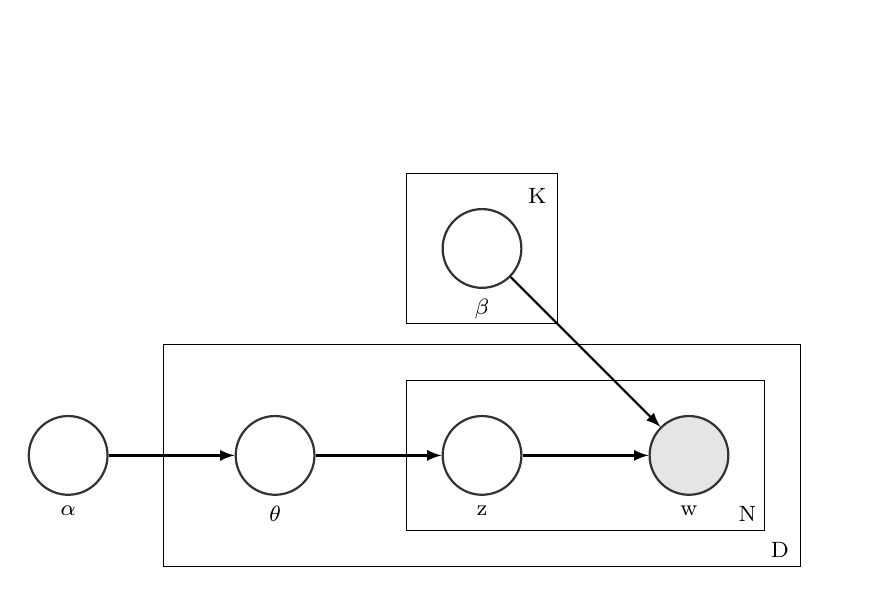
\begin{tikzpicture}
\tikzstyle{main}=[circle, minimum size = 10mm, thick, draw =black!80, node distance = 16mm]
\tikzstyle{connect}=[-latex, thick]
\tikzstyle{box}=[rectangle, draw=black!100]
  % sigma
  \node[main] (alpha) [label=below:$\alpha$] { };    
  % eta
  \node[main] (theta) [right=of alpha,label=below:$\theta$] { };
  % z
  \node[main] (z) [right=of theta,label=below:z] {};
  % beta
  \node[main] (beta) [above=of z,label=below:$\beta$] { };
%  \node[main] (beta) [left=of psi,label=below:$\beta$] { };
  \node[main, fill = black!10] (w) [right=of z,label=below:w] { };
  \path (alpha) edge [connect] (theta)
        (theta) edge [connect] (z)
		(z) edge [connect] (w)
		(beta) edge [connect] (w);
%		(beta) edge [connect] (psi);
  \node[rectangle, inner sep=4.4mm,draw=black!100, fit= (beta)] {};
  \node[rectangle, inner sep=4.4mm, fit= (beta), label=below right:K, xshift=-5mm, yshift=18.5mm] {};
  \node[rectangle, inner sep=0mm, fit= (z) (w),label=below right:N, , xshift=13mm] {};
  \node[rectangle, inner sep=4.4mm,draw=black!100, fit= (z) (w)] {};
    \node[rectangle, inner sep=4.6mm, fit= (z) (w),label=below right:D, xshift=12.5mm] {};
  \node[rectangle, inner sep=9mm, draw=black!100, fit = (theta) (z) (w)] {};
\end{tikzpicture}
\caption{Graphical representation for CTM}
\label{graph:ctm}
\end{figure}
From figure \ref{graph:ctm} we can see, word and topic-word assignment are in the word and document plate $ N\times D $. The document topic proportion $ \eta $ is on the document plate D. Specifically, the topic word proportion $ \beta $ is on the topic plate K, which is specified as word distribution selected by topic assignment z. 

\paragraph{Mathematical Formulation} The joint distribution for CTM is described as follows,
\begin{align*}
p(\eta,z,w|\beta,\mu,\Sigma)=\prod_{d=1}^{D}p(\eta_d|\mu,\Sigma)\prod_{n=1}^{N_d}p(z_{dn}|\eta_d)p(w_{dn}|z_{dn},\beta_{1:K})
\end{align*}
and the ELBO is defined as,
\begin{align*}
\mathcal{L}\geq&\sum_{d=1}^{D}\mathbb{E}_{q_d}\left[\log p(\eta_d,z_d,w_d|\mu,\Sigma,\beta_{1:K})\right]-\sum_{i=1}^{K}\log\text{KL}(q(\eta_i|\lambda_i,\nu_i^2)|p(\eta_d|\mu,\Sigma))\\
&-\sum_{n=1}^{N}\log\text{KL}(q(z_n|\phi_n)||p(z_n|\eta_d))
\end{align*}
\subsection{Embedded Topic Model} \label{ch2:etm}
Embedded Topic Model \cite{dieng_topic_2019} is one of the state-of-art approaches for topic model task. It takes word distribution $ \beta $ as a topic embedding for words. % explain the algorithm
Similar to Word2Vec\cite{mikolov_distributed_nodate}, the word distribution is a softmax function of the inner product of context matrix $ \rho $ and context embedding $ \alpha $. Specifically, the algorithm   equation \ref{eq:etm_embedding}
\begin{equation}\label{eq:etm_embedding}
\beta\sim\sigma(\rho^\top\alpha)
\end{equation}
The word is drawn from the generative process shown in algorithm \ref{algorithm:etm}, for each document, sample a topic distribution $ \theta $ from logistic-normal distribution parameterized with zero mean and identity covariance. Then for each word position n, the model sample topic assignment $ z_{dn} $ from categorical distribution $ \theta_d $. Finally, a word is drawn from $ \text{softmax}(\rho^\top\alpha) $ on $ z_{dn} $ the row.\\
\begin{algorithm}[H]\label{algorithm:etm}
\ForEach{document $d\in 1\dots D $}{
Draw document topic distribution $ \theta_d\sim \mathcal{LN}(0,I) $\\
\ForEach{word position $n\in 1\dots N_d $}{
%Generate topic $ z_{d,n}\sim Cat(\eta_d) $\\
Draw topic assignment $ z_{d,n}\sim Cat(\theta_d) $\\
Draw word $ w_{d,n}\sim \sigma(\rho^\top\alpha)_{z_{dn}} $
}}
\caption{Generative Process for ETM}
\end{algorithm}
Although ETM can maintain for Word2Vec training as the embedding for topic modeling, it cannot capture 
\section{Representation learning}
\subsection{Word Embedding} \label{ch2:we}
% explain what is word embeddings
Word embedding\cite{bengio_neural_nodate} is a kind of representation for words from document collections using a vector formulation. The nature of word embedding is that, the words that having similar meaning have a close distance(in most case euclidean distance), and vice versa. For instance, continuous bag-of-words(CBOW) \cite{mikolov_distributed_nodate} is a kind of word embeddings converting bag-of-word in to a vector of n-dimension continuous space, which contains the following formulation,
\begin{align*}
w\sim\text{softmax}(\rho^\top\alpha)
\end{align*}
where $ \rho\in\mathbb{R}^{L\times V} $ is the embedding matrix which a function $ f:\mathbb{R}^V\mapsto\mathbb{R}^{L} $ maps $ V $ vocabularies into $ L $ dimension of continuous vector space. And $ \alpha $ is the context embedding, which conveniently convert the latent dimension L to a custom dimension of continuous embedding space $ \mathbb{R}^{N} $ as $ \tilde{f}:\mathbb{R}^L\mapsto\mathbb{R}^{N} $.
\subsection{Transformer} \label{ch2:transformer}
Transformer\cite{vaswani_attention_nodate} is a popular neural network architecture in natural language processing. To briefly explain Transformer, it is an stacked encoder-decoder architecture. The component that makes transformer stands out of other architectures it the mutli-head self-attention mechanism. 

In this section we only cover the main components of transformer. The details for transformer can be reviewed in author's blog post\footnote{\url{https://ai.googleblog.com/2017/08/transformer-novel-neural-network.html}}.

To define Transformer,
\subsubsection{Scaled Dot Product Attention}
\begin{align*}
\text{Attention}(Q,K,V) = \sigma\left(\frac{QK^T}{\sqrt{d_k}}\right)V
\end{align*}
\begin{align*}
k_i, q_i\sim\mathcal{N}(0,\sigma)\rightarrow\text{Var}\left(\sum_{i=1}^{d_k}q_i\cdot k_i\right)=\sigma\cdot d_k
\end{align*}
\subsubsection{Multi-head attention}
To obtain a big value from a sentence, extending the attention mechanism to multiple head instead of one could 
\begin{align*}
h_i&=Attn(QW_i^Q,KW_i^K,VW_i^V)\\
\text{MHA(Q,K,V)}&=(h_1,\cdots,h_h)W^O
\end{align*}
\begin{figure}
%\includegraphics[width=0.25\linewidth]{fig/transformer}
\caption{Transformer Architecture}
\label{fig:transformer_arch}
\end{figure}
%\subsection{Multi-Head Attention}
%\begin{align*}
%\text{Multihead}(Q,K,V)=\text{Concat}(\text{head}_i,\dots,\text{head}_h)W^O \\
%\text{head}_i = \text{Attention}(QW_i^{Q}, KW_i^K,VW_i^V)
%\end{align*}
\subsubsection{Positional Encoding}
One drawback for Multi-Head Attention block is that it does not consider information about word positioning, 
\[ PE_{(pos,i)} = \begin{cases} 
\sin\left(\frac{pos}{10000^{i/d}model}\right) & \text{if }i \mod 2 = 0 \\
\cos\left(\frac{pos}{10000^{(i-1)/d}model}\right) & \text{otherwise}
       \end{cases}
    \]
    
For the decoder part, we only consider autoregressive Transformer-decoder in the remaining research.
In this chapter, we explore the detail for posterior inference and give specification to how we . In section \ref{ch4:1}, we give definition to the variational inference method that we use to posterior approximation. Then a detailed derivation for the evidence lower bound(ELBO) of our proposed model will be given in section\ref{ch4:2}. Finally, section \ref{ch4:3} will demonstrate the algorithm that to optimization process of the LKJTM.
\section{Posterior Inference}\label{ch4:1}
Since the exact inference of the posterior is intractable in real application, we employed approximation scheme for the posterior inference. The popular approaches are Markov Chain Monte Carlo Method (MCMC) and Variational Inference(VI)\cite{blei_variational_2006,hoffman_stochastic_2013}. Gibbs sampling is one of the MCMC method and it is fast to compute the approximation and easy to the implementation. Then, Variational EM algorithm to be carried out for maximizing the likelihood over all word in corpus in the document. An alternative way to perform estimation is Monte Carlo method.
\subsection{Variational Inference}
Given that posterior approximiation is not alway practical in real world application. Approximation method are necessary to be apply. Their are two main approach for the posterior approximation: Markov Chain Monte Carlo(MCMC) Variational Inference. Variational Inference is a method approximating the posterior in optimization fashion. To give a better intuition, let probability $ p(x) $ depending on a latent variable $ z $ such that $ p(x|z)=\int p(x|z)p(z)dz $. We can turn the following posterior inference problem into a optimization problem. Here we derive the bound and perform optimization,
\begin{align*}
content...
\end{align*}
\subsection{Stochastic Variational Inference}
Stochastic Variational Inference (SVI)\cite{hoffman_stochastic_2013} is a scalable variant of variational inference, which enables mini-batching to split dataset and train for each epochs, then become a standard of optimization for probabilistic models.
Two main improvement are made by the SVI: stochastic optimization and noisy gradient.
% TODO Collapsing parameters
\subsection{Collapsing Parameters}
In original LDA model, the parameter z is responsible for sampling topic assignment for each word position in every single document. Collapsing parameters\cite{srivastava_autoencoding_2017} introduced to reduce the latent variable $ z $ in the generative process in hence to speed up computation.
\begin{align}\label{eq:cp}
w_d\sim\prod_{n=1}^{N_d}\text{Cat}(\sigma(\beta_{w_{dn}}\theta_d))
\end{align}
The trick in equation \ref{eq:cp} rewrite the original LDA word drawing process, and hence define a new evidence lower bound for the topic model.
% TODO Blei's notes
\subsection{Autoencoding Variational Bayes (AEVB)}
Generally when we optimize a variational parameter, it is neceasary to derive a ELBO and then derive the optimization step for gradient descent. While amortized inference latent variable z is parameterized by two inference network  $ \mu_{\phi(x),\sigma_{\phi}(x)} $ .
% TODO UCLA notes
\begin{align}
z = \mathcal{N}(\mu_{\phi}(x_i), \sigma_{\phi}(x_i))
\end{align}
\begin{align}
\mathcal{L}=\mathbb{E}_{z\sim\mathcal{N}(\mu_{\phi}(x_i),\sigma_\phi(x_i))}\left[\log p_\theta(x_i|z)\right]-D_{KL}\left(q_\phi(z|x_i)||p(z)\right)
\end{align}
\subsection{Reparameterization trick}
The drawback of amortized inference is that, sampling from normal distribution parameterizing $ \mu_{\phi(x),\sigma_{\phi}(x)} $ could lead to high variance outcome and hamper the inference performance. For the reason, taking reparamterization trick\cite{kingma_auto-encoding_2014} to transform as equation \ref{eq:rt},
\begin{align}\label{eq:rt}
z= \mu_{\phi}(x_i)+\epsilon\sigma_\phi(x_i)\text{, }\epsilon\sim\mathcal{N}(0,1)
\end{align}
where $ \epsilon $ is a sample from normal distribution $ \mathcal{N}(0,1) $. and so the modified ELBO becomes equation \ref{eq:elbo_rt},
\begin{align}\label{eq:elbo_rt}
\mathcal{L}=\mathbb{E}_{\epsilon\sim N(0,1)}\left[\log p_\theta(x_i|\mu_{\phi}(x_i)+\epsilon\sigma_\phi(x_i))\right]-D_{KL}\left(q_\phi(z|x_i)||p(z)\right)
\end{align}
\section{Evaluation metrics}
\subsection{Perplexity}The proposed model will be evaluated with perplexity metric. The metric will examine how well the model can tackle with unseen data. It is equivalent algebraically to the inverse of the geometric mean per-word likelihood. Lower perplexity scores mean better.\begin{equation*}
\text{Perplexity}(D_{test})=\exp{{-\frac{\sum_{d=1}^{M}\sum_{m=1}^{N_d}\log p(w_{dm})}{\sum_{d=1}^{M}N_d}}}
\end{equation*}
\subsection{Topic Coherence}Topic Coherence\cite{mimno_optimizing_2011} measures the quality of the topic 
\begin{equation*}
TC=\frac{1}{K}\sum_{k=1}^{K}\frac{1}{45}\sum_{i=1}^{10}\sum_{j=i+1}^{10}f(w_i^{(k)},w_j^{(k)})\end{equation*}
where $\{w_1^{(k)},\cdots,w_{10}^{(k)}\}$ denotes top-10 most likely words in topic k. And function $f(\cdot,\cdot)$ is te normalized pointwise mutual information.\begin{equation*}
f(w_i,w_j)=\frac{\log\frac{P(w_i,w_j)}{P(w_i)P(w_j)}}{-\log P(w_i,w_j)}\end{equation*}
\subsection{Topic Diversity} In order to compare how the words each topic are differentiate the others. We applied the Topic Diversity metric \cite{dieng_topic_2019}. Topic Diversity (TD) to be the percentage of unique words in the top 25 words of all topics. Diversity close to 0 indicates redundant topics; diversity close to 1 indicates more varied topics. We define the overall metric for the quality of a model’s topics as the product of its topic diversity and topic coherence.
\begin{align*}
TD=\frac{|A\cap B|}{|A \cup B|}
\end{align*}
where $ A $ and $ B $ are top-k words from two topics. 
\chapter{Model Formulation}\label{ch3}
In this chapter, we give a detailed explanation and procedure of LKJTM to be implemented.
\section{Model description}
The TETM utilizes the Transformer as embedding to the topic-word representations. To compare with the original topic model, the word-topic distribution $ \beta $ is the 
First, the topic embedding embeds the vocabulary into L-dimensional space, which is by Transformer embedding. Second, the context embedding maps the embedding into K-dimensional space . 
In the generative process, the LKJTM uses the topic embedding to form a per-topic vector to represent the meaning over the vocabulary. 
% Generative process
The generative process of the $ d^{th} $ document is the following:\\
\begin{algorithm}[H]
\For{document d in D}{
Sample topic distribution $ \theta_d\sim \mathcal{LN}(0,I) $\\
\For{word position n in $ N_d $}{
Sample word $ w_{d,n}\sim \sigma(\theta_d(\rho^\top\alpha)_{\cdot,w_{d,n}}) $
}
}
\caption{Generative Process for TETM}
\label{algorithm:lkjtm}
\end{algorithm}
From algorithm \ref{algorithm:lkjtm}, starting from step 1, the topic proportion $ \theta_d $ is drawn from the logistic-normal distribution $ \mathcal{LN}(\cdot) $ with zero mean and identical covariance.
From Step 2-a, for each word position $ n $ in document $ d $, a topic assignment to word $ w_{dn} $ is drawn from categorical distribution $ Cat(\theta_d) $ parameterized by topic proportion $ \theta_d $
Step 2-b, the model draw a word from embedding of the vocabulary $ \rho $ and the assigned topic embedding $ \alpha_{z_{dn}} $ to draw the observed word from the assigned topic, as given by $ z_{dn} $. The embedding is applied softmax function to make them topic distribution.
The TETM likelihood uses a matrix of word embedding $ \rho $, a representation of the vocabulary in a lower dimensional space. In practice, it can either rely on previously fitted embeddings as part of the fitting procedure, it simultaneously finds topics and an embedding space.

% TODO LKJ Correlation Distribution Formulation

% TODO Transformer Embeddings
% Transformer embeddings
\subsection{Transformer Embeddings}
Following the ETM architecture, we modify topic-word distribution as an embedding and put transformer embedding to work into it. 
\begin{equation}\label{eq:transformer_embedding}
\beta\sim\text{softmax}(\rho^\top\alpha)
\end{equation}
Equation \ref{eq:transformer_embedding}, 
%% Joint Distribution
\subsection{Joint Distribution}
We give a description of the joint distribution, $ W,Z,\theta $ and $ \Sigma $ are variables and $ \beta, \mu $ and $ \gamma $ are latent variables. $ W $ is the word likelihood from the document collections, $ Z $ represents the topic-word assignment, $ \theta $ models the topic distribution for each document, and $ \Sigma $ is the covariance matrix which depends on the document-topic distribution $ \theta $.
\begin{align*}
p(w,\theta,\alpha)=\prod_{d=1}^{D}\int p(\theta_d)\prod_{i=1}^{N_d}p(w|\theta_d,\alpha)d\theta_d
\end{align*}
by taking  log on the joint probability, we obtain a objective function for optimization
% Marginal Likelihood
\subsection{Marginal Likelihood}
The parameter $ \alpha $ is the topic embedding on the word embedding space of dimension K. We take a log marginal likelihood of the document,
\begin{align*}
\mathcal{L}(\alpha)=\sum_{d=1}^{D}\log p(w_d|\alpha)
\end{align*}
\begin{align*}
p(w_d|\alpha)=\int p(\theta_d|\mu,\Sigma)\prod_{n=1}^{N_d}p(w_{dn}|\theta_d,\alpha)d\theta_d
\end{align*}
the conditional distribution $ p(w_{dn}|\theta_d,\alpha) $ marginalize out the the topic assignment $ z_{dn} $,
\begin{align*}
p(w_{dn}|\theta_d,\alpha)=\sum_{k=1}^{K}\theta_{dk}\beta_{k,w_{dn}}
\end{align*}
where $ \beta $ represent the topic-word distribution, composed of transformer embedding $ \rho $ and topic embedding $ \alpha $, in such case
\begin{align*}
\beta_{kv}=\text{softmax}(\rho^\top\alpha)_{v}.
\end{align*}
then we take the amortized inference to take out neural network for the representation,
\begin{align*}
p(w_{d}|N(\mu_\theta(w),\sigma_\theta(w)),\beta)=\mathbb{E}_{\theta\sim N(\mu_\theta(w),\sigma_\theta(w))}\left[w^\top\sigma(\beta\theta)\right]
\end{align*}
Reparametrization Trick $ \theta=\mu+\sigma^{1/2}\epsilon $\\
\begin{align*}
p(w_{d}|\mu_\theta(w)+\epsilon\sigma^{1/2}_\theta(w),\beta)=\mathbb{E}_{\epsilon\sim N(0,1)}\left[w_d^\top\sigma(\beta(\mu_\theta(w)+\epsilon\sigma^{1/2}_\theta(w)))\right]
\end{align*}
\chapter{Inference and Estimation}\label{ch4}
In this chapter, we explore the detail for posterior inference and give specification to how we . In section \ref{ch4:1}, we give definition to the variational inference method that we use to posterior approximation. Then a detailed derivation for the evidence lower bound(ELBO) of our proposed model will be given in section\ref{ch4:2}. Finally, section \ref{ch4:3} will demonstrate the algorithm that to optimization process of the LKJTM.
\section{Posterior Inference}\label{ch4:1}
Since the exact inference of the posterior is intractable in real application, we employed approximation scheme for the posterior inference. The popular approaches are Markov Chain Monte Carlo Method (MCMC) and Variational Inference(VI)\cite{blei_variational_2006,hoffman_stochastic_2013}. Gibbs sampling is one of the MCMC method and it is fast to compute the approximation and easy to the implementation. Then, Variational EM algorithm to be carried out for maximizing the likelihood over all word in corpus in the document. An alternative way to perform estimation is Monte Carlo method.
\subsection{Variational Inference}
Given that posterior approximiation is not alway practical in real world application. Approximation method are necessary to be apply. Their are two main approach for the posterior approximation: Markov Chain Monte Carlo(MCMC) Variational Inference. Variational Inference is a method approximating the posterior in optimization fashion. To give a better intuition, let probability $ p(x) $ depending on a latent variable $ z $ such that $ p(x|z)=\int p(x|z)p(z)dz $. We can turn the following posterior inference problem into a optimization problem. Here we derive the bound and perform optimization,
\begin{align*}
content...
\end{align*}
\subsection{Stochastic Variational Inference}
Stochastic Variational Inference (SVI)\cite{hoffman_stochastic_2013} is a scalable variant of variational inference, which enables mini-batching to split dataset and train for each epochs, then become a standard of optimization for probabilistic models.
Two main improvement are made by the SVI: stochastic optimization and noisy gradient.
% TODO Collapsing parameters
\subsection{Collapsing Parameters}
In original LDA model, the parameter z is responsible for sampling topic assignment for each word position in every single document. Collapsing parameters\cite{srivastava_autoencoding_2017} introduced to reduce the latent variable $ z $ in the generative process in hence to speed up computation.
\begin{align}\label{eq:cp}
w_d\sim\prod_{n=1}^{N_d}\text{Cat}(\sigma(\beta_{w_{dn}}\theta_d))
\end{align}
The trick in equation \ref{eq:cp} rewrite the original LDA word drawing process, and hence define a new evidence lower bound for the topic model.
% TODO Blei's notes
\subsection{Autoencoding Variational Bayes (AEVB)}
Generally when we optimize a variational parameter, it is neceasary to derive a ELBO and then derive the optimization step for gradient descent. While amortized inference latent variable z is parameterized by two inference network  $ \mu_{\phi(x),\sigma_{\phi}(x)} $ .
% TODO UCLA notes
\begin{align}
z = \mathcal{N}(\mu_{\phi}(x_i), \sigma_{\phi}(x_i))
\end{align}
\begin{align}
\mathcal{L}=\mathbb{E}_{z\sim\mathcal{N}(\mu_{\phi}(x_i),\sigma_\phi(x_i))}\left[\log p_\theta(x_i|z)\right]-D_{KL}\left(q_\phi(z|x_i)||p(z)\right)
\end{align}
\subsection{Reparameterization trick}
The drawback of amortized inference is that, sampling from normal distribution parameterizing $ \mu_{\phi(x),\sigma_{\phi}(x)} $ could lead to high variance outcome and hamper the inference performance. For the reason, taking reparamterization trick\cite{kingma_auto-encoding_2014} to transform as equation \ref{eq:rt},
\begin{align}\label{eq:rt}
z= \mu_{\phi}(x_i)+\epsilon\sigma_\phi(x_i)\text{, }\epsilon\sim\mathcal{N}(0,1)
\end{align}
where $ \epsilon $ is a sample from normal distribution $ \mathcal{N}(0,1) $. and so the modified ELBO becomes equation \ref{eq:elbo_rt},
\begin{align}\label{eq:elbo_rt}
\mathcal{L}=\mathbb{E}_{\epsilon\sim N(0,1)}\left[\log p_\theta(x_i|\mu_{\phi}(x_i)+\epsilon\sigma_\phi(x_i))\right]-D_{KL}\left(q_\phi(z|x_i)||p(z)\right)
\end{align},
% Inference Equation
% Variational Inference
% KL-divergence for the logistic normal distribution
\section{Evidence Lower Bound(ELBO)}\label{ch4:2} To perform Variational inference, it is essential to derive the Evidence Lower Bound (ELBO) first as the objective function for the optimization. By 
\begin{align}\label{eq:elbo_1}
\mathcal{L}\geq&\mathbb{E}_q[\log p(W,Z,\theta,\Sigma)]-\mathbb{E}_q[\log q(Z,\theta,\Sigma)]\\
=&\sum_{d=1}^{D}\sum_{n=1}^{V}\mathbb{E}_q[\log p(w_{d,n}|z_{d,n},\beta)]+\sum_{d=1}^{D}\sum_{n=1}^{V}\mathbb{E}_q[\log p(z_{d,n}|\theta_d)]\\
&+\sum_{d=1}^{D}\mathbb{E}[\log p(\theta_d|\mu,\Sigma)]+\mathbb{E}_q[\log p(\Sigma|\gamma)]-\sum_{d=1}^{D}\sum_{n=1}^{V}\mathbb{E}_q[\log q(z_{d,n}|\alpha_{d,n})]\\
&-\sum_{d=1}^{D}\mathbb{E}_q[\log q(\theta_d|\lambda_d,\nu_d)]-\mathbb{E}_q[\log q(\Sigma|\phi)]
\end{align}
% TODO Monte Carlo Estimate
The expectation log likelihood term in \ref{eq:elbo_1} can be efficiently appriximated by the Monte Carlo sampling method,
\begin{align}\label{eq:elbo_2}
\mathcal{L}\approx\frac{1}{S}\sum_{s=1}^{S}p(W|\theta^{(s)})
\end{align}
\paragraph{Collapsing Parameters}
\begin{align}\label{eq:elbo_3}
\mathcal{L}&\geq\sum_{d=1}^{D}\int\int q(\theta_d)\log\frac{p(W_d|\theta_d,\beta)p(\theta_d|\mu,\Sigma)p(\Sigma|\gamma)}{q(\theta_d)q(\Sigma)}d\theta_d d\Sigma\\
&=\sum_{d=1}^{D}\left(\mathbb{E}_{q(\theta_d)}\left[\log p(W_d|\theta_d,\beta)\right]-KL(q(\theta_d)||p(\theta_d|\mu,\Sigma))\right)-KL(q(\Sigma)||p(\Sigma|\gamma))
\end{align}
Here we define amortized inference, a optimization technique which perform inference by defined neural networks. $ \mu_\theta(w) $ and $ \sigma_\theta(w) $ are two inference networks take input from the word $ w $. Then a output is generated by the Normal distribution parameterized by $ \mu_\theta(w) $ and $ \sigma_\theta(w) $.
\begin{align}\label{eq:elbo_4}
=&\sum_{d=1}^{D}\left(\mathbb{E}_{q(\theta_d)}\left[\log p(w_d|\mathcal{LN}(\mu_{\theta_d}(w_d),\sigma_{\theta_d}(w_d)),\beta)\right]-KL(q(\theta_d)||p(\theta_d|\mu,\Sigma))\right)\\
&-KL(q(\Sigma)||p(\Sigma|\gamma))
\end{align}
To apply reparameterization trick, we take transformation from normal distribution to $ \theta=\mu+\epsilon\sigma^{1/2} $ where $ \epsilon\sim N(0,1) $, as  equation \ref{eq:elbo_5}
\begin{align}\label{eq:elbo_5}
=&\sum_{d=1}^{D}\left(\mathbb{E}_{q(\epsilon)}\left[\log p(w_d|\sigma(\mu_{\theta_d}(w_d)+\epsilon\sigma_{\theta_d}(w_d)),\beta)\right]-KL(q(\theta_d)||p(\theta_d|\mu,\Sigma))\right)\\
&-KL(q(\Sigma)||p(\Sigma|\gamma))
\end{align}
we also apply the minibatch to make able the model perform by subsampling the document collection. By equation \ref{eq:elbo_6}
\begin{align}\label{eq:elbo_6}
\tilde{\mathcal{L}}=&\frac{\mathcal{D}}{|\mathcal{B}|}\sum_{d\in\mathcal{D_B}}\left(\mathbb{E}_{q(\epsilon)}\left[\log p(w_d|\sigma(\mu_{\theta_d}(w_d)+\epsilon\sigma_{\theta_d}(w_d)),\beta)\right]-KL(q(\theta_d)||p(\theta_d|\mu,\Sigma))\right)\\
&-KL(q(\Sigma)||p(\Sigma|\gamma))
\end{align}
The KL-divergence for the logistic-normal distribution is given as equation \ref{eq:elbo_7} closed-form expression,
\begin{align}\label{eq:elbo_7}
\text{KL}(q(\theta_d)||p(\theta_d|\mu,\Sigma))=-\frac{1}{2}\left(tr(\sigma_1^{-1}\sigma_0)+(\mu_1-\mu_0)\Sigma_1^{-1}(\mu_1-\mu_0)-K+\log\frac{|\sigma_1|}{|\sigma_0|}\right)
\end{align}
so the ELBO then becomes \ref{eq:elbo_8}
\begin{align}\label{eq:elbo_8}
\tilde{\mathcal{L}}=&\sum_{d=1}^{D}\left[-\frac{1}{2}\left(tr(\sigma_1^{-1}\sigma_0)+(\mu_1-\mu_0)\Sigma_1^{-1}(\mu_1-\mu_0)-K+\log\frac{|\sigma_1|}{|\sigma_0|}\right)\right]\\
&+\mathbb{E}_{\epsilon\sim\mathcal{N}(0,I)}\left[w_d^\top\log\sigma(\beta(\mu_0+\sigma_0^{1/2}\epsilon))\right]-KL(q(\Sigma)||p(\Sigma|\gamma))
\end{align}
% TODO Transformer Loss
\section{Transformer Loss}
It is suggested that using cross entropy loss for transformer training. In equation \ref{eq:crossentropy}, . It is worth mention that, the 
\begin{align}\label{eq:crossentropy}
L_{\text{CrossEntropy}}=-\frac{1}{V}\sum_{i=1}^{V}y_i\cdot\log(\hat{y_i})
\end{align}
% TODO algorithm for the optimization here
\section{Optimization step}\label{ch4:3}
In algorithm \ref{algorithm:lkjtm_obj}, first initialize the model and variational parameters. Then, for each epochs, we obtain the transformer embedding $ \rho $ from transformer. After that, the topic embedding $ \beta $ is computed by taking softmax of dot-product of $ \rho $ and $ \alpha $. Then a minibatch $ \mathcal{B} $ is selected from the document for optimization. The number of minibatch is the document collection divides minibatch size where $ \#\text{minibatch}=\frac{\mathcal{D}}{|\mathcal{B}|} $. For each minibatch, the model takes a document and sample lower Cholesky matrix from LKJ Cholesky distribution(description see section \ref{ch2:lkj}). A topic assignment for document d $ \theta_d $ is sampled from logistic-normal distribution $ \mathcal{LN}(\mu,\sigma LL^\top\sigma) $, where $ \mu $ is sampled from half-Cauchy distribution and covariance is a transformation from equation \ref{eq:lkj_trans}. For each word position n, a word is sampled from the softmax of dot-product of transformer embedding $ \rho $ and NN weight $ \alpha $. After the sampling process for the document collection, we estimate the ELBO loss $ L_{ELBO} $ for the topic model, and the cross entropy loss $ L_{CrossEntropy} $. Remind that the topic model and transformer take input differently. The topic model part takes bag-of-words input, a document-vocabulary matrix $ D\times V $ counting the occurrence of vocabulary v in document d. While transformer take sequence of document as input. 
To calculate the loss of the model , we sum up the ELBO loss $ L_{ELBO} $ and cross entropy loss for transformer $ L_{CrossEntropy} $. Then a stochastic gradient is computed by backpropagation. a gradient step to . The process iterates until the maximum iteration is reached. 
\\
\begin{algorithm}[H]
Initialize model and variational parameters\\
\For{epoch $i=1,2,\dots N$}{
Compute the trnasformer embedding $ \rho $\\
Compute $ \beta=\text{softmax}(\rho^\top\alpha) $\\
Choose a minibatch $ \mathcal{B} $ of documents\\
\ForEach{document d in $ \mathcal{B} $}{
Compute $ \mu_d=\text{NN}(x_d;\nu_\mu) $\\
Compute $ \sigma_d=\text{NN}(x_d;\mu_\sigma) $\\
Sample $ L\sim \text{LKJChol}(\gamma) $ \\
Sample $\theta_d\sim\mathcal{LN}(\mu,\sigma LL^\top\sigma)$\\
\ForEach{word position n in docuemnt $ N_d $}{
Sample word $ w_{dn}\sim \text{softmax}(\beta_{w_{dn}}\theta_{d}) $
}
}
Estimate ELBO loss $ \text{L}_\text{ELBO}$ from Eq. \ref{eq:elbo_8}\\
Compute Transformer loss $ \text{L}_\text{CrossEntropy}$ from Eq. \ref{eq:crossentropy}\\
Compute the total loss $ \text{L}=\text{L}_\text{ELBO}+\text{L}_\text{CrossEntropy} $\\
Compute the stochastic gradient via backpropagation\\
Take a stochastic gradient step\\
Update model parameters ($\rho,\alpha,$)\\
Update variational parameters ($ \ $)
}
\label{algorithm:lkjtm_obj}
\caption{Topic modeling with the LKJTM}
\end{algorithm}
%\begin{algorithm}[H]
%Initial $ \theta^{(0)} $ randomly\\
%\While{Not Converge}{
%Sample a document d uniformly from dataset $ \mathcal{D} $\\
%For all k, initial $ \gamma^{d}_{k}=1 $\\
%\While{Not Converge}{
%\For{$ i=1,\cdots,N_d $}{
%\begin{align*}
%\phi_{ik}^{d}\propto\exp{\mathbb{E}}[\log\pi^d_k]+\mathbb{E}[\log\beta_{k,w_i^d}]
%\end{align*}
%}
%Set $ \gamma^{d}=\alpha+\sum_{i=1}^{N_d}\phi_i^d $
%}
%Take a stochastic gradient step $ \theta^{t}=\theta^{t-1}+\epsilon_t+\triangledown_\theta\mathcal{L}_d $
%}
%\caption{SVI for LDA}
%\end{algorithm}
\chapter{Results \& Evaluations}\label{ch5}
In this chapter, we perform evaluation on our model and the other algorithms, the repository of our model is provided in github \footnote{\url{https://github.com/cwleung/LKJTM}}.
\section{Experiment Testing}
The experiment will be conducted with a number of existing proposed topic models as mentioned related work section above. We conduct the experiment with those baseline algorithms and evaluate them in terms of accuracy and running time. Some of the source code of competitive were provided by their authors in Github\footnote{For instance, Correlated Topic Model (CTM), \href{https://github.com/blei-lab/ctm-c}{https://github.com/blei-lab/ctm-c}}. The outcome result will be extensively studied and conclude the insight behind the algorithms and methodologies. Detail to be stated in section \ref{AD}.
\section{Algorithmic Settings}
% optimization algorithm
To perform posterior inference, we employed Stochastic Variational Inference (SVI) \cite{hoffman_stochastic_2013} for the optimization problem. We set the minibatch size to 1024 documents.
% Other model
For LDA, we applied the model provided from sklearn package (version 0.24.0) \footnote{Sklearn website \url{https://scikit-learn.org/stable/index.html}}. For ETM, we run the experiment with the parameter suggested \cite{dieng_topic_2019}. For ProdLDA, we perform optimization with inference network architecture as described in the paper \cite{srivastava_autoencoding_2017}. 
% learning rate
To perform optimization, we use Adam for the gradient ascent algorithm, and we set the learning rate to 1e-3.
% l2-regularization factor
we use $ \mathcal{l-2} $ regularization to the 
% inference network [size, activation function, dropout, batch-norm]
We use 
% Transformer settings

% 
\section{Dataset}To evaluate the performance of the model, we select the two most poplar data set in the context of topic model evaluation. 20Newsgroups and Reuter RCV1-v2 datasets. 20NewsGroup consist of 18,846 news group documents \footnote{\url{http://qwone.com/~jason/20Newsgroups/}} and the RCV1-v2 includes 10,000 documents in total. Both of the dataset will be preprocessed to remove stopwords and stemming before the evaluation. If desirable, it will also to be applied to NIST TREC dataset and NII NTCIR dateset for further application studies.
\section{Data Preprocessing}
We perform data preprocessing, tokenization, stopword removal, lemmatization, and set the 
\section{Models}
We compare the model performance with a numbers of rivals. We take Latent Dirichlet Allocation (LDA) as the baseline model.
\section{Quantitative Result}
In this section, we evaluate the model with the following metric adopted from \cite{dieng_dynamic_2019}: Perplexity, Topic Coherence (TC), Topic Diversity (TD). %and Topic Quality (TQ).\begin{center}
\paragraph{Perplexity}The proposed model will be evaluated with perplexity metric. The metric will examine how well the model can tackle with unseen data. It is equivalent algebraically to the inverse of the geometric mean per-word likelihood. Lower perplexity scores mean better.\begin{equation*}
\text{Perplexity}(D_{test})=\exp{{-\frac{\sum_{d=1}^{M}\sum_{m=1}^{N_d}\log p(w_{dm})}{\sum_{d=1}^{M}N_d}}}
\end{equation*}
\paragraph{Topic Coherence}Topic Coherence \cite{mimno_optimizing_2011}
\begin{equation*}
TC=\frac{1}{K}\sum_{k=1}^{K}\frac{1}{45}\sum_{i=1}^{10}\sum_{j=i+1}^{10}f(w_i^{(k)},w_j^{(k)})\end{equation*}
where $\{w_1^{(k)},\cdots,w_{10}^{(k)}\}$ denotes top-10 most likely words in topic k. And function $f(\cdot,\cdot)$ is te normalized pointwise mutual information.\begin{equation*}
f(w_i,w_j)=\frac{\log\frac{P(w_i,w_j)}{P(w_i)P(w_j)}}{-\log P(w_i,w_j)}\end{equation*}
\paragraph{Topic Diversity} In order to compare how the words each topic are differentiate the others. We applied the Topic Diversity metric \cite{dieng_topic_2019}. Topic Diversity (TD) to be the percentage of unique words in the top 25 words of all topics. Diversity close to 0 indicates redundant topics; diversity close to 1 indicates more varied topics. We define the overall metric for the quality of a model’s topics as the product of its topic diversity and topic coherence.
\begin{align*}
TD=\frac{|A\cap B|}{|A \cup B|}
\end{align*}
where $ A $ and $ B $ are top-k words from two topics. 
% \paragraph{Topic Quality}
\begin{table}[]
\centering
\begin{tabular}{llll}
\hline
Model      & TC     & Perplexity  \\ \hline
Transformer & -0.311 & - \\
LDA & 0.183 & 2425.9 \\
ProdLDA		&  0.107 & 5652.0\\
ETM	     	&  0.177 & \textbf{1919.3}\\
\textbf{Our model}  & \textbf{0.206} & 3444.1 \\ \hline
\end{tabular}
\caption{Result of our implementation(topic k=20)}
\end{table}
\begin{table}[]
\centering
\begin{tabular}{llll}
\hline
Model      & TC     & Perplexity  \\ \hline
Transformer & -0.251 & - \\
LDA & 0.155 & \textbf{2536.1} \\
ProdLDA		&  0.074 & 5654.1\\
ETM	     	&  0.145 & 2603.9\\
\textbf{Our model}  & \textbf{0.199} & 3705.0 \\ \hline
\end{tabular}
\caption{Result of our implementation(topic k=50)}
\end{table}
\section{Qualitative Result}The proposed model will be evaluated with a number of specifically selected topic and examined with their performance separately. The result will be exhaustively compared with other existing models.
\begin{table}[]
\centering
\begin{tabular}{llll}
\hline
ETM  \\ \hline
space, nasa, gov, mr, president, health, research, year, center\\
windows, file, window, program, files, server, version, dos, image\\
god, people, jesus, christian, israel, bible, jews, christians, israeli\\
key, encryption, chip, clipper, keys, privacy, security, technology, government\\
gun, people, government, law, state, guns, article, weapons, control
\\ \hline
ETM  \\ \hline
space, nasa, gov, mr, president, health, research, year, center\\
windows, file, window, program, files, server, version, dos, image\\
god, people, jesus, christian, israel, bible, jews, christians, israeli\\
key, encryption, chip, clipper, keys, privacy, security, technology, government\\
gun, people, government, law, state, guns, article, weapons, control
\\ \hline
ETM  \\ \hline
space, nasa, gov, mr, president, health, research, year, center\\
windows, file, window, program, files, server, version, dos, image\\
god, people, jesus, christian, israel, bible, jews, christians, israeli\\
key, encryption, chip, clipper, keys, privacy, security, technology, government\\
gun, people, government, law, state, guns, article, weapons, control
\\ \hline
ETM  \\ \hline
space, nasa, gov, mr, president, health, research, year, center\\
windows, file, window, program, files, server, version, dos, image\\
god, people, jesus, christian, israel, bible, jews, christians, israeli\\
key, encryption, chip, clipper, keys, privacy, security, technology, government\\
gun, people, government, law, state, guns, article, weapons, control
\\ \hline
ETM  \\ \hline
space, nasa, gov, mr, president, health, research, year, center\\
windows, file, window, program, files, server, version, dos, image\\
god, people, jesus, christian, israel, bible, jews, christians, israeli\\
key, encryption, chip, clipper, keys, privacy, security, technology, government\\
gun, people, government, law, state, guns, article, weapons, control
\\ \hline
\end{tabular}
\caption{Testing}
\end{table}
\subsection{Visualization}
To clearly demonstrate the representation for , we applied t-SNE to map the topic-word representation into 2-dimension continuous space. In figure \ref{fig:tsne50t25w0}, .
%\begin{figure}
%\centering
%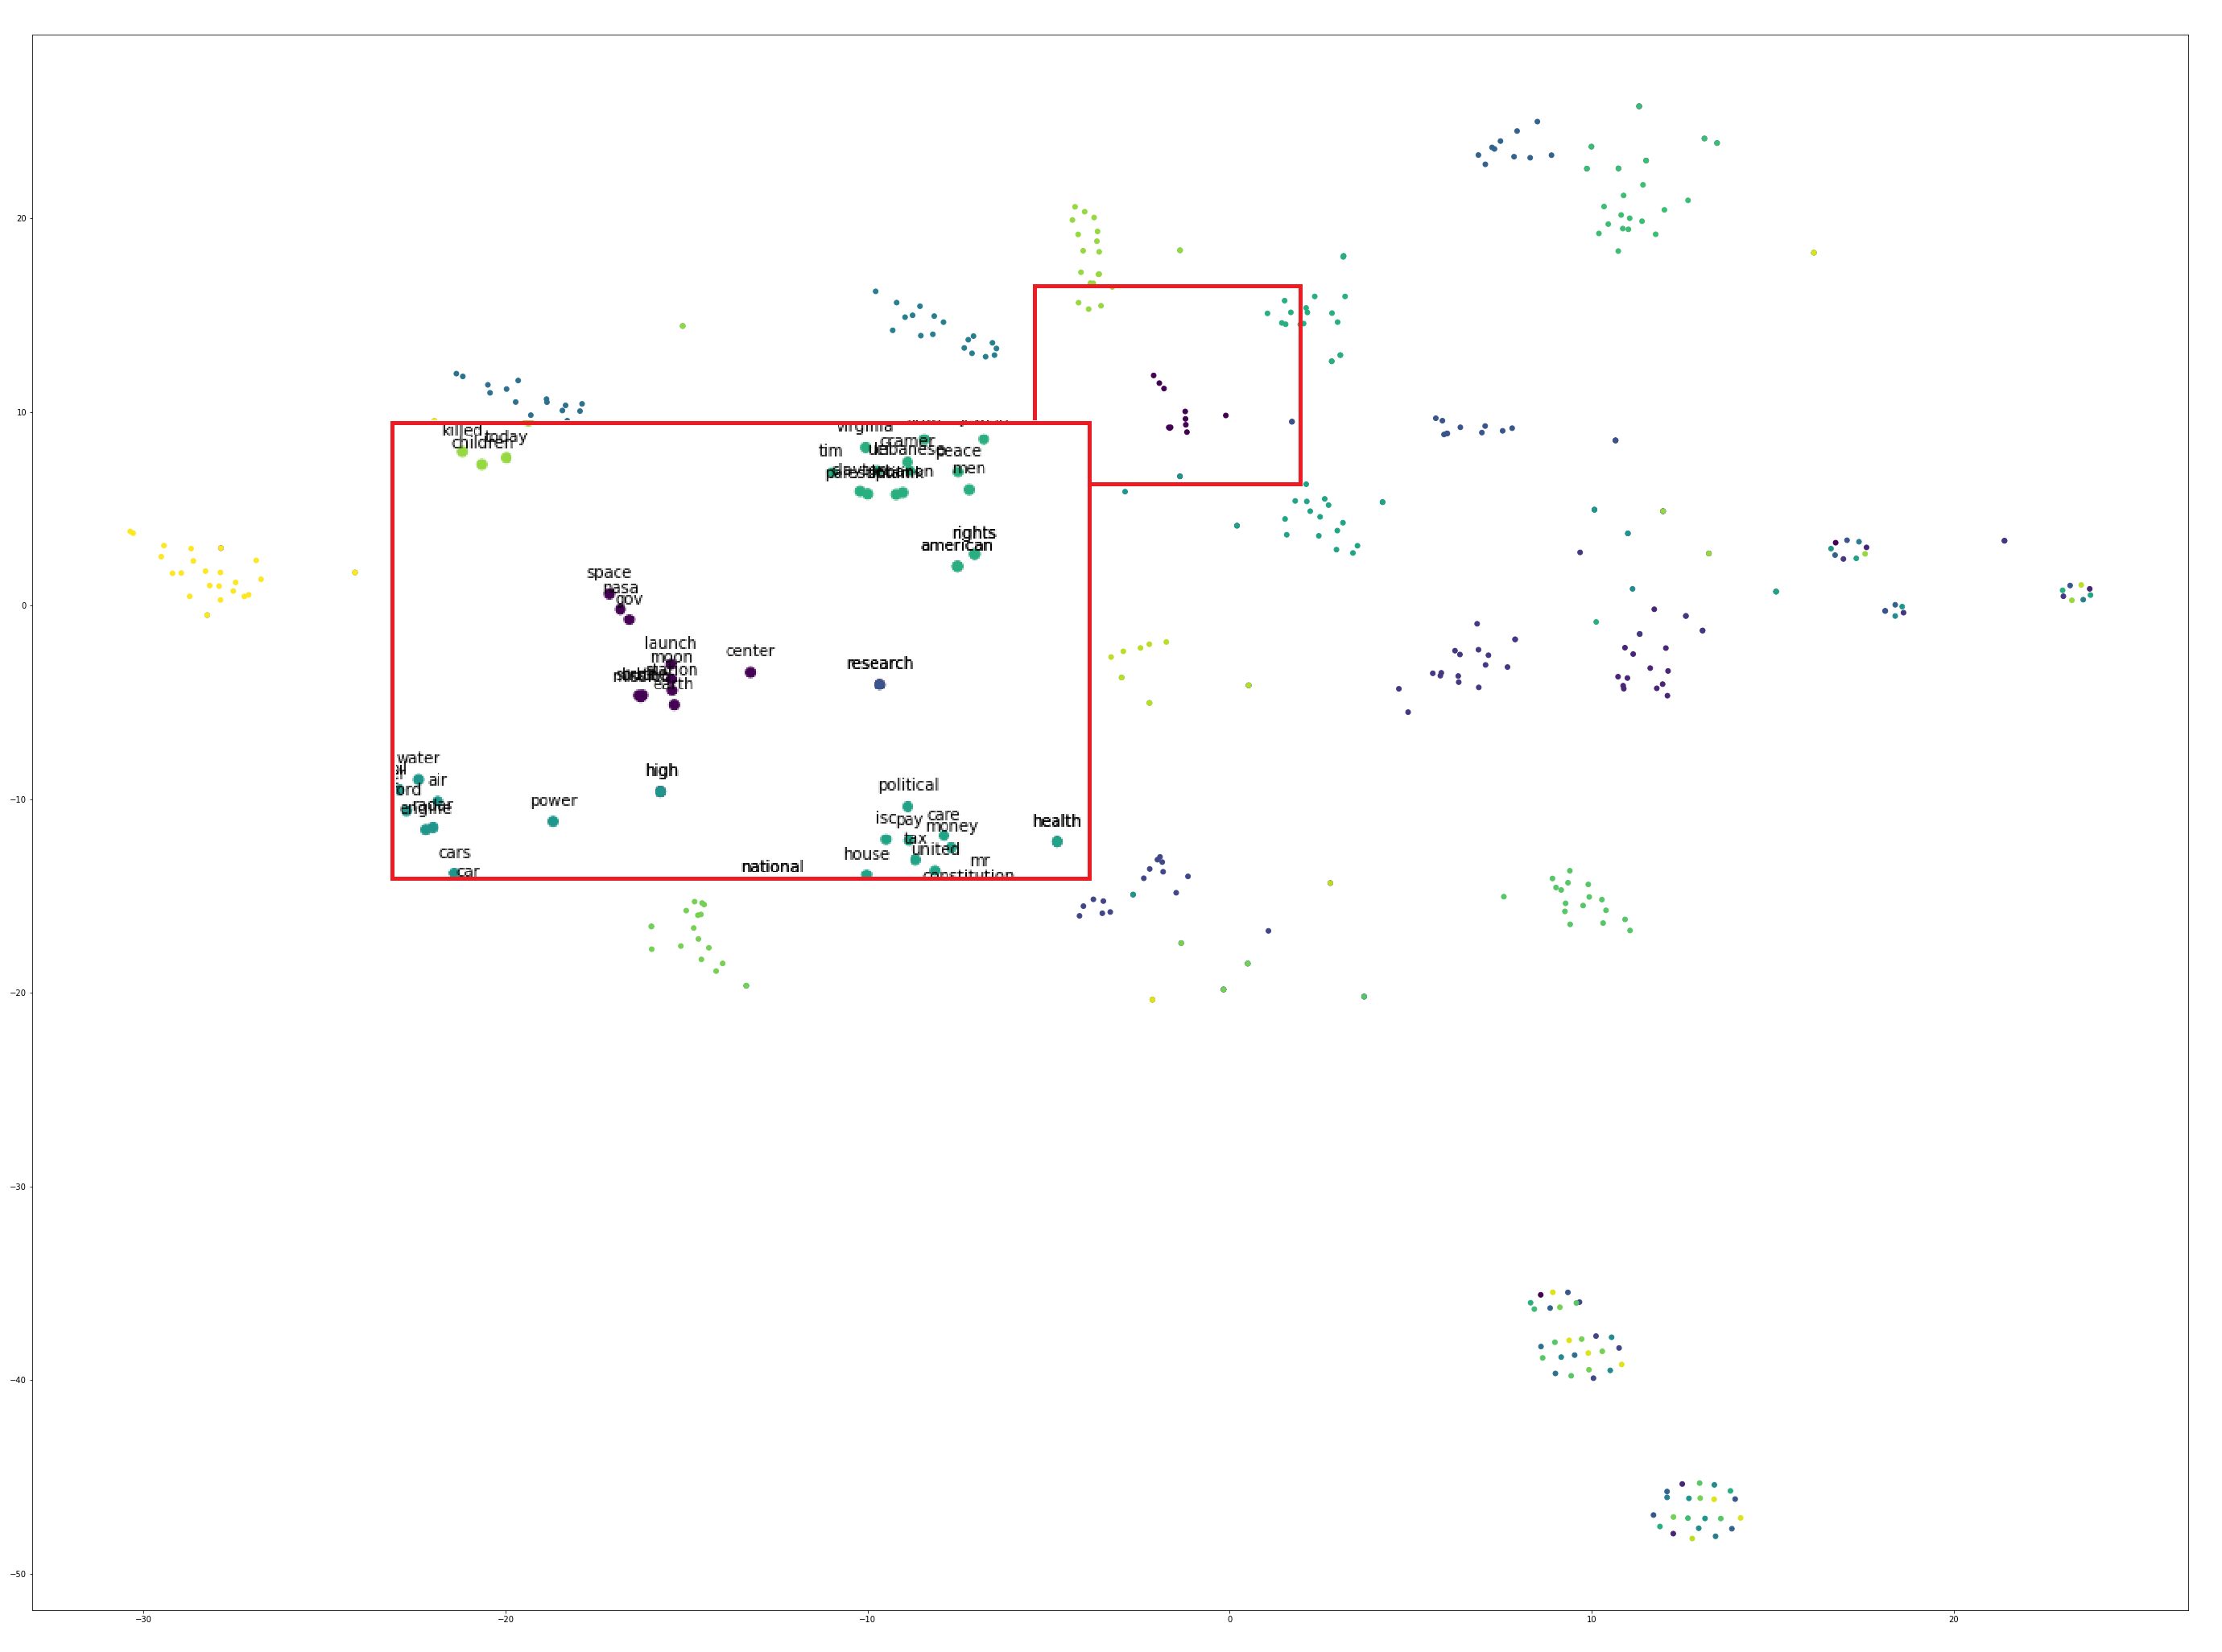
\includegraphics[width=1\linewidth]{figure/tsne_20t_25w_2}
%\caption{Visualization \#Topics:20}
%\label{fig:tsne20t25w2}
%\end{figure}
%\begin{figure}
%\centering
%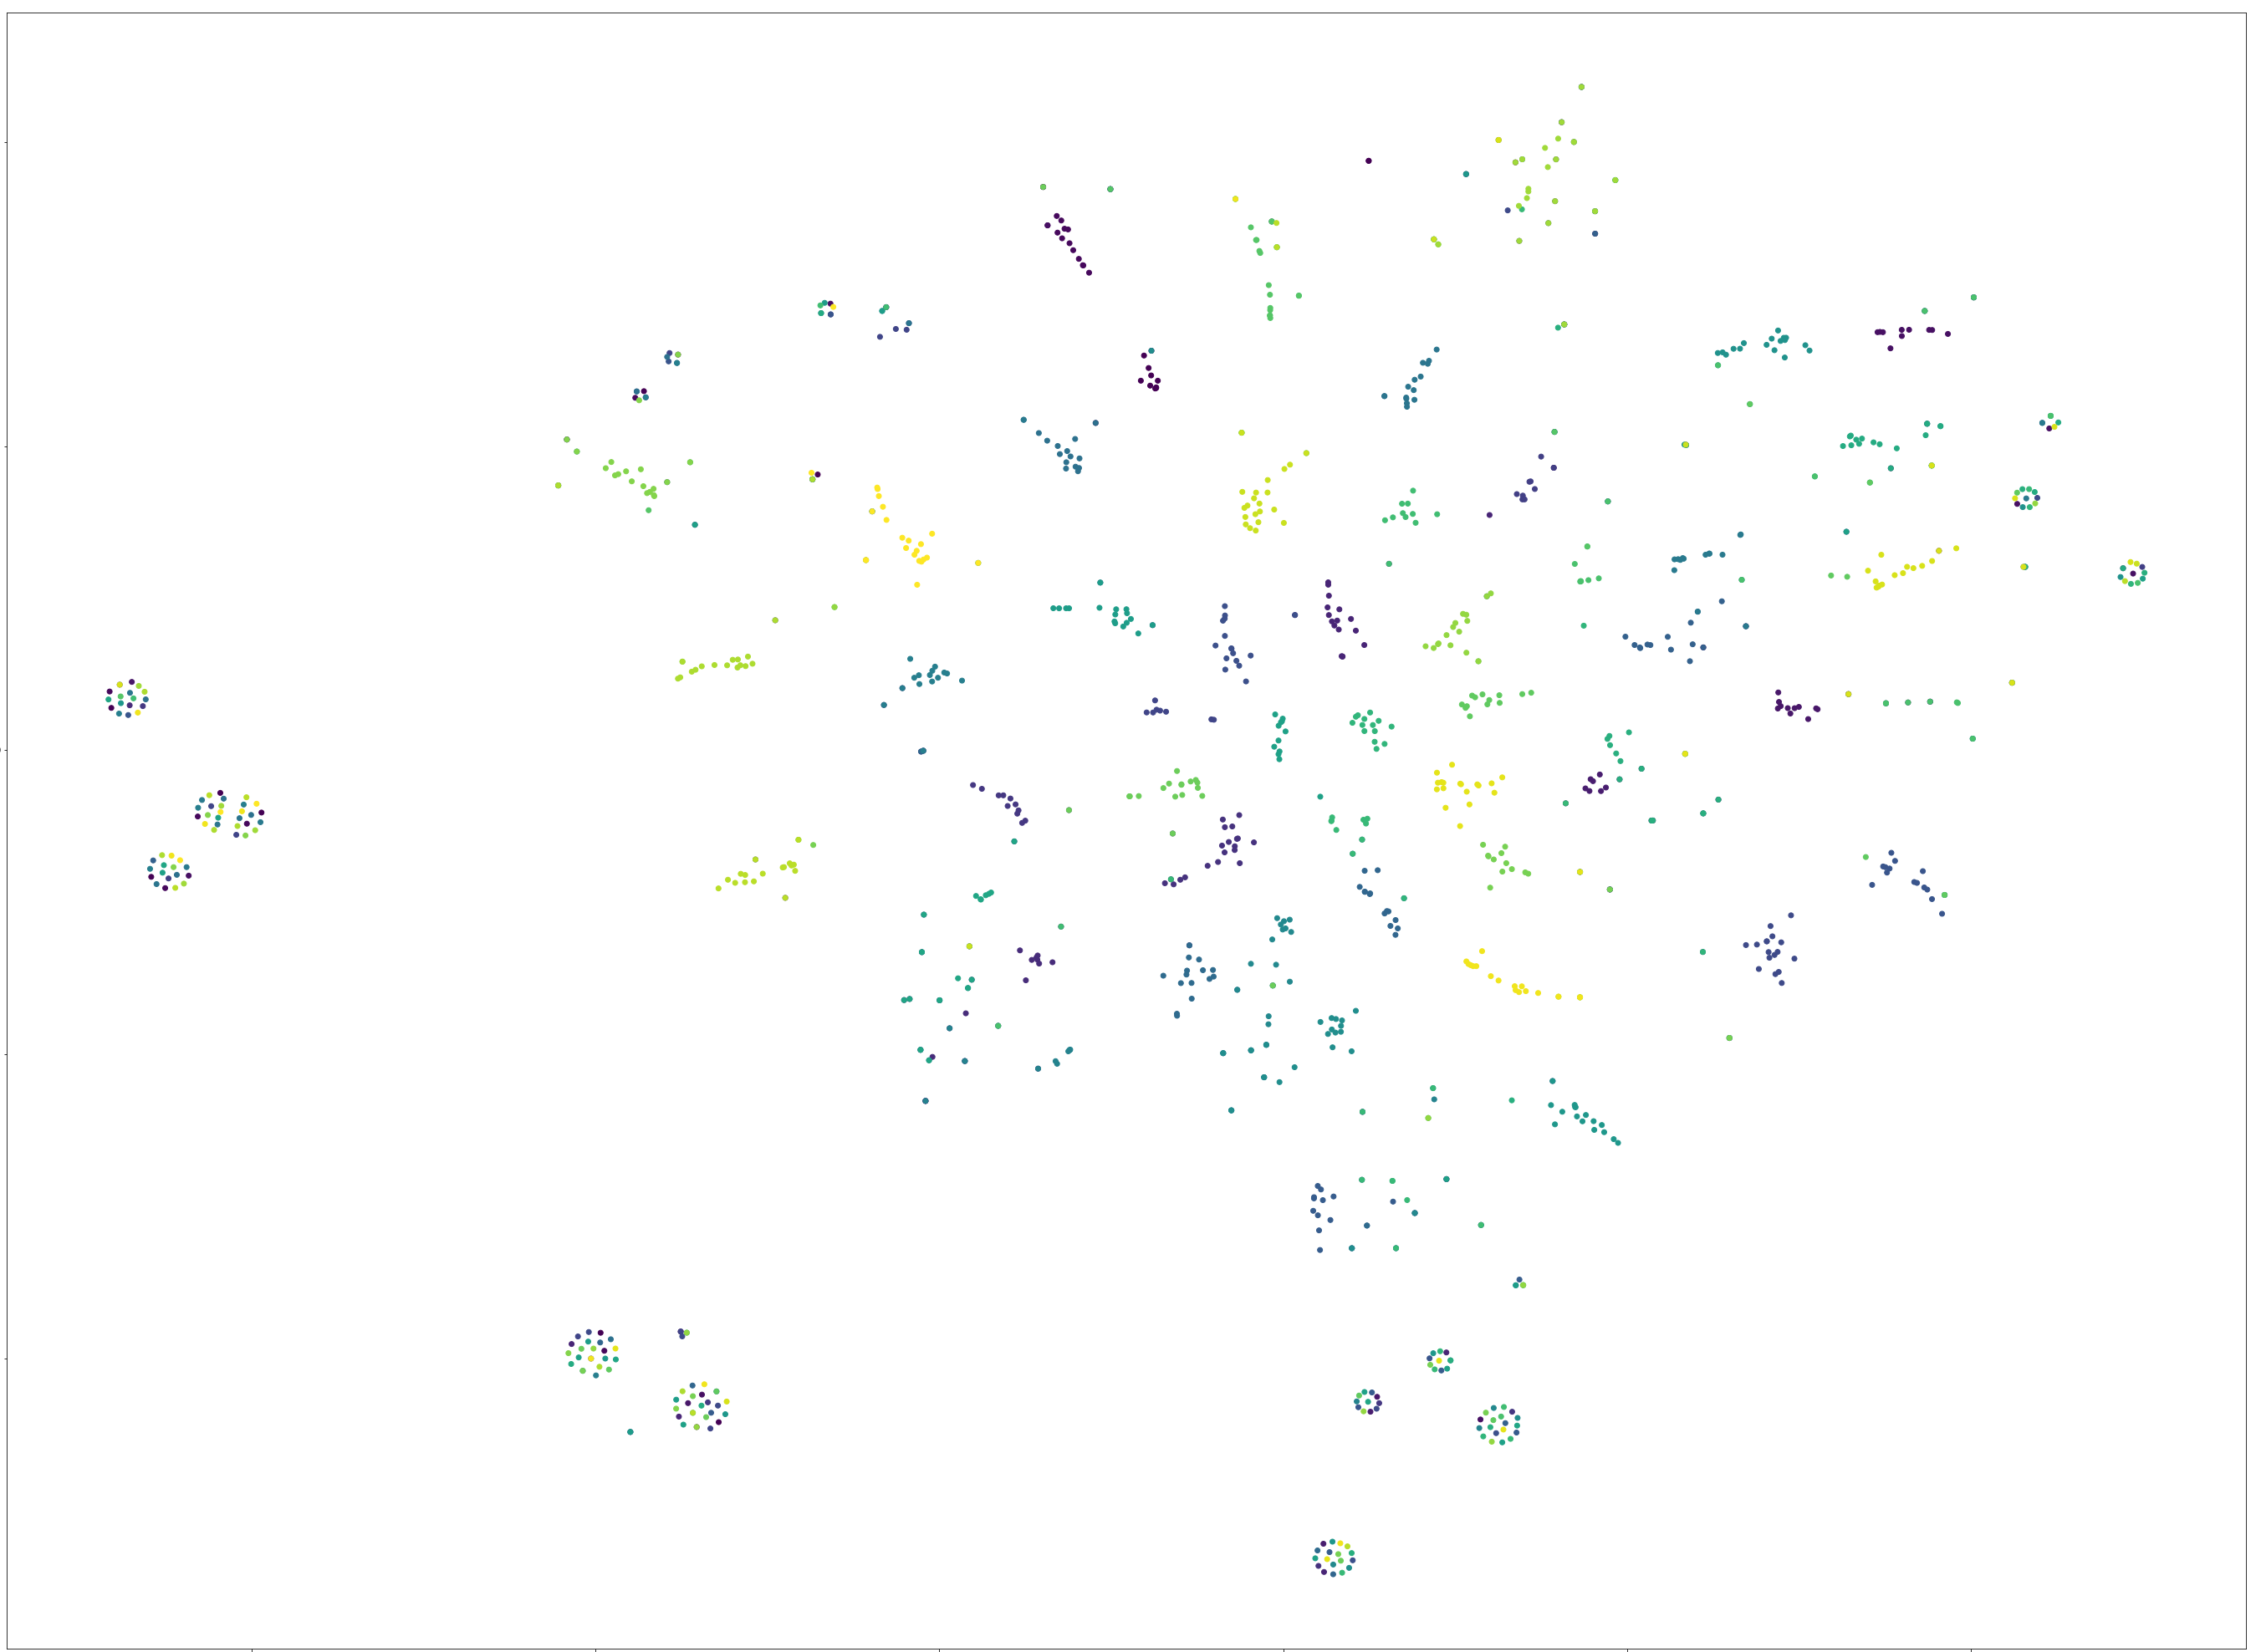
\includegraphics[width=1\linewidth]{figure/tsne_50t_25w_0}
%\caption{Visualization \#Topics:50}
%\label{fig:tsne50t25w0}
%\end{figure}

\chapter{Conclusion}\label{ch6}
In this paper, we proposed a topic model with transformer embedding. The result has shown a better performance in returning high quality topics compared with other state-of-the-art models. Our model also demonstrates a capability in classifying substantial number of topics.
%-------------------
\cite{wallach_rethinking_nodate}
\bibliographystyle{plain} % ŽQl•¶Œ£
\bibliography{thesis} %
%-------------------
%\appendix
%\chapter{Latent Dirichlet Allocation}
%\section{Latent Dirichlet Allocation (LDA)} Latent Dirichlet Allocation\cite{blei_latent_2003} is one of the popular latent variable model. It is found extensively useful in finding hidden topic model in a massive document set. The model is inspired by probabilistic semantic analysis (pLSA)\cite{hofmann_probabilistic_2013} and its naming was taken in a similar sense.
In the following, the LDA model will be explain with graphical model approach. In the figure,This define a joint posterior distribution $p(\theta,z,\beta|w)$. \begin{itemize}
\item $z_d$, $n$ is the per-word topic assignment.
\item $\theta_d$ is the per-document topic proportion.
\item $\theta_k$ is the per-corpus topic distribution.
\end{itemize}
\begin{figure}
\centering
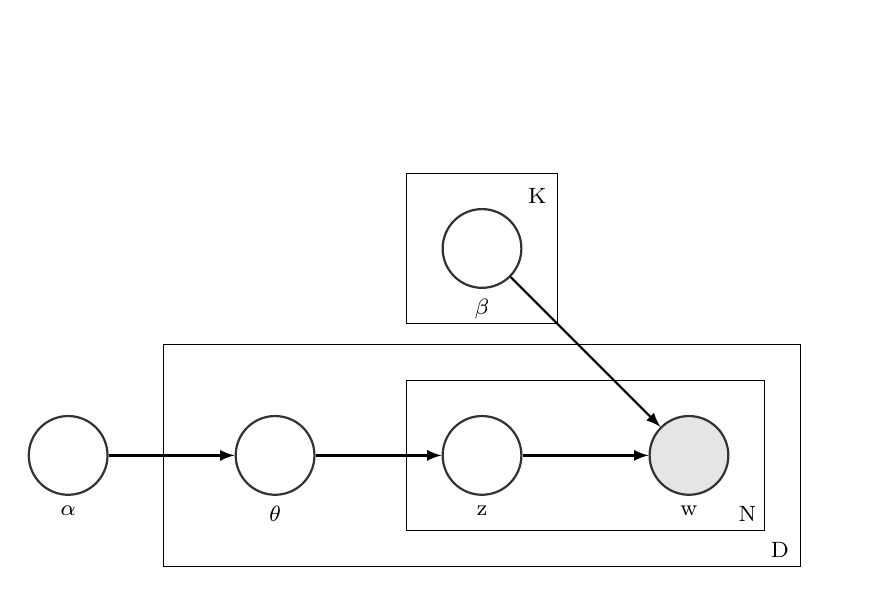
\begin{tikzpicture}
\tikzstyle{main}=[circle, minimum size = 10mm, thick, draw =black!80, node distance = 16mm]
\tikzstyle{connect}=[-latex, thick]
\tikzstyle{box}=[rectangle, draw=black!100]
  % sigma
  \node[main] (alpha) [label=below:$\alpha$] { };    
  % eta
  \node[main] (theta) [right=of alpha,label=below:$\theta$] { };
  % z
  \node[main] (z) [right=of theta,label=below:z] {};
  % beta
  \node[main] (beta) [above=of z,label=below:$\beta$] { };
%  \node[main] (beta) [left=of psi,label=below:$\beta$] { };
  \node[main, fill = black!10] (w) [right=of z,label=below:w] { };
  \path (alpha) edge [connect] (theta)
        (theta) edge [connect] (z)
		(z) edge [connect] (w)
		(beta) edge [connect] (w);
%		(beta) edge [connect] (psi);
  \node[rectangle, inner sep=4.4mm,draw=black!100, fit= (beta)] {};
  \node[rectangle, inner sep=4.4mm, fit= (beta), label=below right:K, xshift=-5mm, yshift=18.5mm] {};
  \node[rectangle, inner sep=0mm, fit= (z) (w),label=below right:N, , xshift=13mm] {};
  \node[rectangle, inner sep=4.4mm,draw=black!100, fit= (z) (w)] {};
    \node[rectangle, inner sep=4.6mm, fit= (z) (w),label=below right:D, xshift=12.5mm] {};
  \node[rectangle, inner sep=9mm, draw=black!100, fit = (theta) (z) (w)] {};
\end{tikzpicture}
\caption{Graphical representation for LDA}
\label{graph:lda}
\end{figure}
The mathematical formulation for LDA as follows.
\begin{itemize}
\item Joint Distribution for LDA
\begin{equation*}
\prod_{i=1}^{K}p(\beta_i)\left[\prod_{d=1}^{D}p(\theta_d)\prod_{n=1}^{N}p(z_{d,n}|\theta_d)p(w_{d,n}|\beta_{1:K},z_{d,n})\right]
\end{equation*} 
\item conditioning on $w_{1:D}$
\begin{equation*}
p(\beta_{1:K},\theta_{1:D},z_{1:D}|w_{1:D})=\frac{p(\beta_{1:K},\theta_{1:D},z_{1:D},w_{1:D})}{p(w_{1:D})}
\end{equation*}
\end{itemize}
\begin{algorithm}[H]
Initialize hyperparameters $ \alpha $, $ \beta $\\
\For{topic k in K}{
Sample a word distribution $ \phi_k\sim \text{Dir}(\beta) $
}
\For{document d in D}{
Sample a topic distribution $ \theta_d\sim \text{Dir}(\alpha) $\\
\For{word position n in $ N_d $}{
Sample a topic assignment $ z_{dn}\sim \text{Cat}(\theta_d) $\\
Sample a word $ w_{dn}\sim \text{Cat}(\phi_{z_{dn}}) $
}
}
\caption{Generative Process for LDA}
\end{algorithm}
The procedure for LDA as follows. For each topic k$\in$\{1,...,K\}, draw a multinomial distribution $\beta_k$ from a Dirichlet distribution with parameter $\lambda$. For each document d$\in$\{1,...,M\}, draw a multinomial distribution $\theta_d$ from a Dirichlet distribution with parameter $\alpha$. For each word position n$\in$\{1,...,N\}, select a topic $z_n$ from the Multinomial distribution parameterized by $\theta_d$. Choose the observed word $w_n$ from the distribution $\theta_{z_n}$.

%-------------------
\end{document}
